\subsection{Erkennungsregeln deployen und nutzen}
\label{sec:deploying_recognitionrules}

Um die Erkennungsregeln zu testen, gibt es zwei Möglichkeiten:

\begin{enumerate}

\item Eclipse Application: 
Öffnen Sie die \texttt{MANIFEST.MF} des Projekts der Erkennungsregeln und starten sie über das \textit{Launch Icon} (vgl. Abb. \ref{silift-rulebase_run_eclipse_application}) eine zweite Eclipse-Instanz. Innerhalb dieser Instanz sind alle Projekte aus Ihrem Workspace registriert und können verwendet werden.

\begin{figure}[H]
\centering
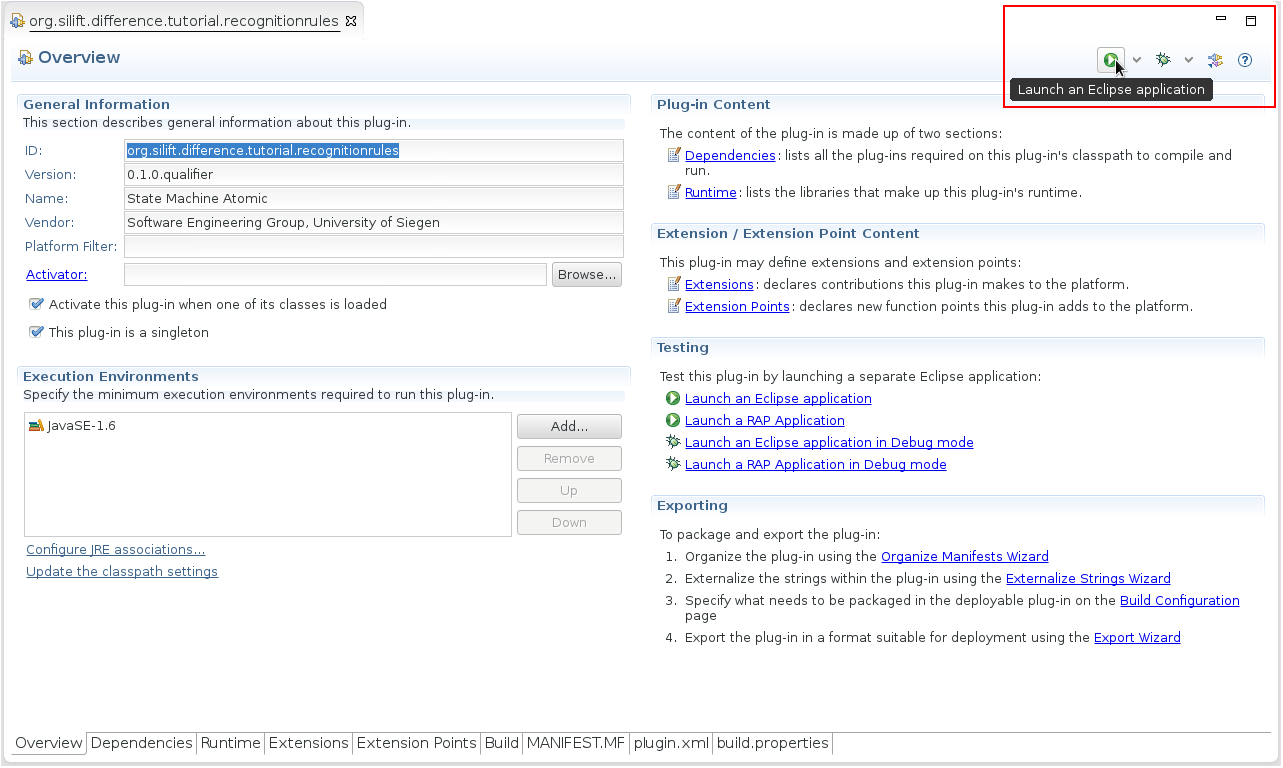
\includegraphics[width=0.8\textwidth]{recognitionrules/graphics/silift-rulebase_run_eclipse_application.png}
\caption{Run Ecplipse Application}
\label{silift-rulebase_run_eclipse_application}
\end{figure}


\item Deployable Plugins and Fragments: analog zu Abschnitt \ref{sec:own_matching_engine}.
\end{enumerate}

Wenn Sie Ihre Regeln erstmal nur testen möchten, ist die erste Variante zu bevorzugen. 
Sofern Sie die zweite Variante nutzen und ggf. mit Hilfe des \textit{Rulebase-Managers} an den Erkennungsregeln  etwas verändern möchten, müssen Sie die installierten Plugins zuerst deinstallieren.\\

Eine umfassende Einführung in die Nutzung von SiLift als Differenzwerkzeug finden Sie im \textbf{SiLift - Benutzerhandbuch für Endanwender}.